\chapter{先行研究}
\label{chap:prior}
本論文の議論のベースとなる,岡田らの従来手法と
島田らが提案したトポロジカルマップの形式,単語の組み合わせで経路を表現したシナリオについて述べる

\section{視覚と行動のend-to-end学習により経路追従行動を
オンラインで模倣する手法}
岡田らの従来手法について述べる.
岡田らの従来手法では,メトリックマップに基づくナビゲーションの経路追従行動をend-to-end学習により,
視覚を入力とした行動へ模倣する.
これにより,視覚に基づくナビゲーションを獲得できる.
手法に基づいて構築されたシステムを\figref{fig:okada_sys}に示す.

まずはじめに学習器の訓練を行う.
学習器の訓練時,LiDARやオドメトリを入力とするメトリックマップに基づく
ルールベース制御器を用いて,設定した経路を追従する.
その際,ロボットに取り付けた,カメラから得たRGB画像とルールベース制御器が出力する
ヨー方向の角速度をペアとして0.2秒の周期でデータセットへ加える.
次にデータセットから,バッチサイズを8として教師データを抽出し,0.2秒の周期で
end-to-end学習する.
このデータセットへのデータの追加から学習までの1連の流れを1ステップとしている.
カメラ画像の収集には,3つのカメラを用いる.
左右のカメラ画像に対するヨー方向の角速度は,経路に戻るようなオフセット(\(\pm 0.2\)rad/s)を加える.

学習器の訓練後は,学習器へ中央のカメラから得たRGB画像を入力し,出力されるヨー方向の角速度を用いて経路を追従する.
この時,並進速度は0.2m/sの一定の値を用いる.
\vspace{10zh}
\begin{figure}[htbp]
    \centering
     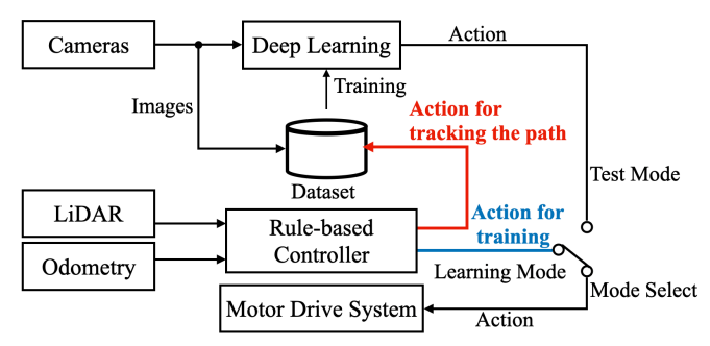
\includegraphics[width=110mm]{images/pdf/okada_method_sys.pdf}
     \caption[Structure of the Okada and others proposed system]{Structure of the Okada and others proposed system(Quoted from\cite{okada2020})}
     \label{fig:okada_sys}
\end{figure}
\clearpage
この岡田らの従来手法は,ルールベース制御器を教師データの収集に用いることで,
データセットの収集に人間の操作が不要となること,
\figref{fig:robo_ac}に示すように学習のデータセットに加える行動と
学習時にロボットを制御する行動を別々に
扱うことで,常に経路に戻る行動のみをデータセットに追加できるといった特長がある.
\begin{figure}[htbp]
    \centering
     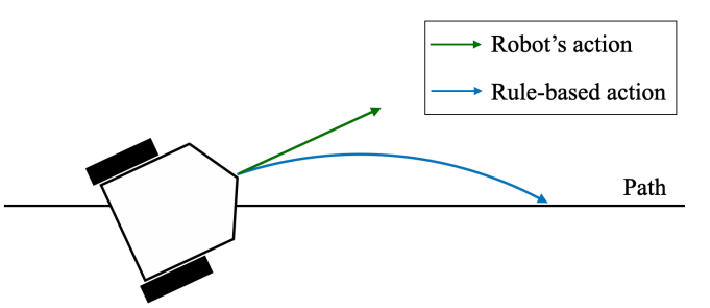
\includegraphics[width=100mm]{images/pdf/robo_action.pdf}
     \caption[Rule-based actions
     apart from the robot's actions]{Rule-based actions
     apart from the robot's actions(Quoted from\cite{okada2020})}
     \label{fig:robo_ac}
\end{figure}

\figref{fig:okada_net}
に岡田らの従来手法における学習器のネットワーク構造を示す.
ネットワークは,入力層 1,畳み込み層 3,全結合層 2,出力層 1 の全7層で構成される.
活性化関数としてReLU\cite{relu},最適化アルゴリズムにAdam\cite{adam},
損失関数としてSoftmax-cross-entropyを用いる.
学習器は入力を64x48のRGB画像データ,出力をロボットのヨー方向の角速度として
end-to-end学習する.
\begin{figure}[htbp]
    \centering
     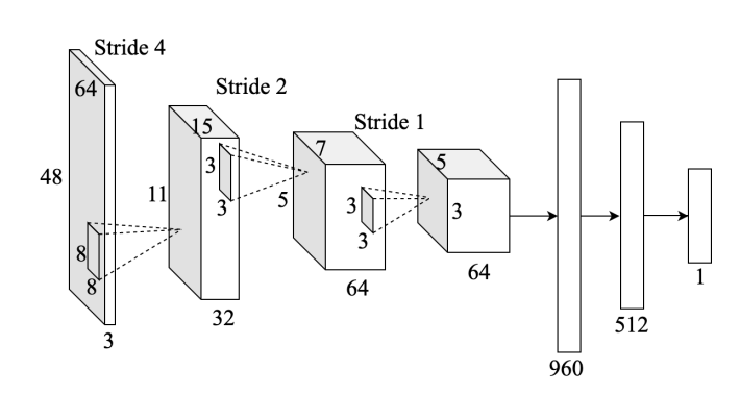
\includegraphics[width=100mm]{images/pdf/okada_network.pdf}
     \caption[Structure of the network used in the method of Okada and others]{Structure of the network used in the method of Okada and others(Quoted from \cite{okada2020})}
     \label{fig:okada_net}
\end{figure}

\clearpage
\section{トポロジカルマップとシナリオ}
\label{sec:shimada_topo_sce}
ここでは,分岐路で適切な進行方向を提示する機能のベースとなる,
島田ら\cite{shimada2020}が提案したトポロジカルマップの形式とシナリオについて述べる.
\subsection{トポロジカルマップ}
% \label{subsec:shimada_topo}
トポロジカルマップは,環境中のランドマークなどの
特徴的な箇所(ノード)とその繋がり(エッジ)によって
環境を表現したマップである.
島田らは\figref{fig:topo}に示すようなトポロジカルマップの形式\cite{shimada2020}を提案している.
島田らのトポロジカルマップでは,ノードは通路の特徴的な箇所に配置され,エッジはそれらのノードを接続するように配置される.
ノードにはID,通路の特徴(Type),エッジのIDと相対角度(Edge)のデータ,エッジにはIDのデータのみが含まれている.
このトポロジカルマップの形式は,人の道案内に関するアンケートを実施し,その結果に基づいて決定された.
アンケートでは,人は道案内において「通路の特徴」や「向いている方向」を重視していることが明らかになっている.
% 人の道案内のデータを収集・解析し,
% その結果から通路の特徴や向きに関する言葉が多用されたことに基づいて決定された.
% 該当する位置に配置され,
% その位置がどのような通路の特徴であるかという情報を
% 持っている.また,「直進」や「右折」といった~で述べるシナリオの行動から
% 移動するエッジを選択するために,ノードはエッジのIDと相対角度の情報を
% 持っている.エッジはノードの接続関係を表すように
% ノード同士を結んでいる.多くの研究では距離に関する情報を持っていることが
% 多いが,島田らの形式ではIDのみを持っている.
% 本稿で用いるトポロジカルマップは,島田らが提案した形式を指す.
% \vspace{5zh}
\begin{figure}[htbp]
    \centering
     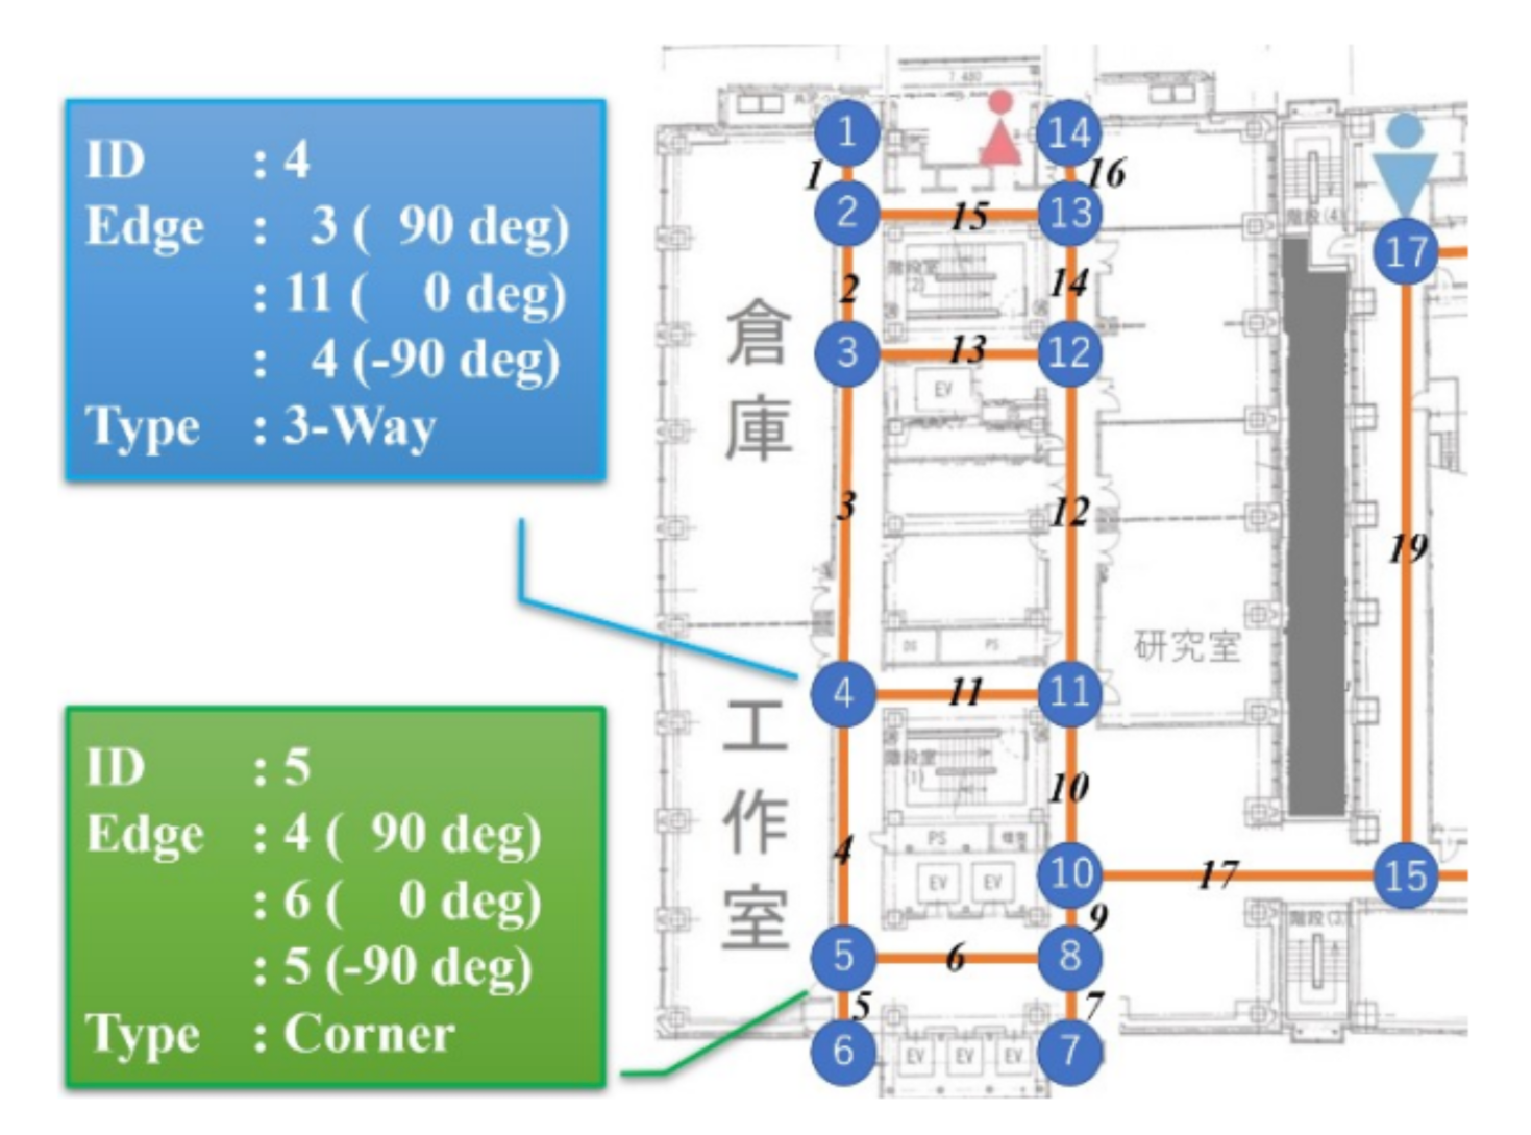
\includegraphics[width=90mm]{images/pdf/topo.pdf}
     \caption[Topological map format proposed by Shimada and others]{Topological map format proposed by Shimada and others(Quoted from\cite{shimada2020})}
     \label{fig:topo}
\end{figure}
\clearpage
\subsection{シナリオ}

シナリオはトポロジカルマップ上での,目的地までの経路を単語の組み合わせで表現したものである.
具体的には,「次の角」や「突き当たりまで」のような「条件」と「直進」,「右折」のような「行動」の組み合わせにより作成される.
このシナリオの形式は,前述のトポロジカルマップと同様に人の道案内に関するアンケートを実施し
,その結果に基づいて決定された.
アンケートでは,人は「条件」と「行動」を組み合わせて道案内をしていることが明らかになっている.
例として,\figref{fig:scenario01}に示す経路をシナリオで表現すると,「3番目の三叉路まで直進.停止」となる.

\vspace{3zh}
\begin{figure}[htbp]
    \centering
     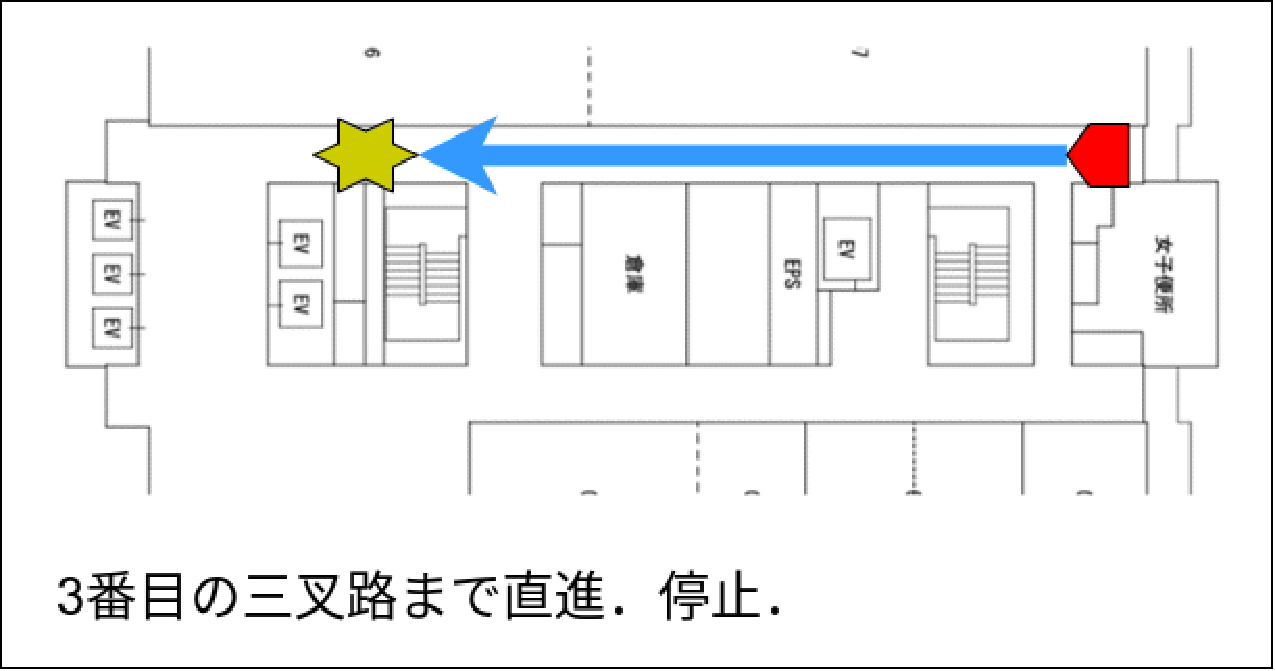
\includegraphics[width=110mm]{images/pdf/scenario/scenario01.pdf}
     \caption[Example scenarios]{Example scenarios(Quoted from \cite{haruyama2023})}
     \label{fig:scenario01}
\end{figure}